\label{generalBehavior}

El sistema final se muestra en la figura \ref{fig:spaceinvblock}. El sistema cuenta con los bloques básicos requeridos por el enunciado de la práctica, así como una serie de bloques extra añadidos como mejora del diseño básico. Estos bloques se explicarán de forma detallada en la sección \ref{blocksexplanation}, junto a las razones tras su implementación y cómo se llevaron a cabo las pruebas de los distintos bloques.

\begin{figure}[H]
	\centering
	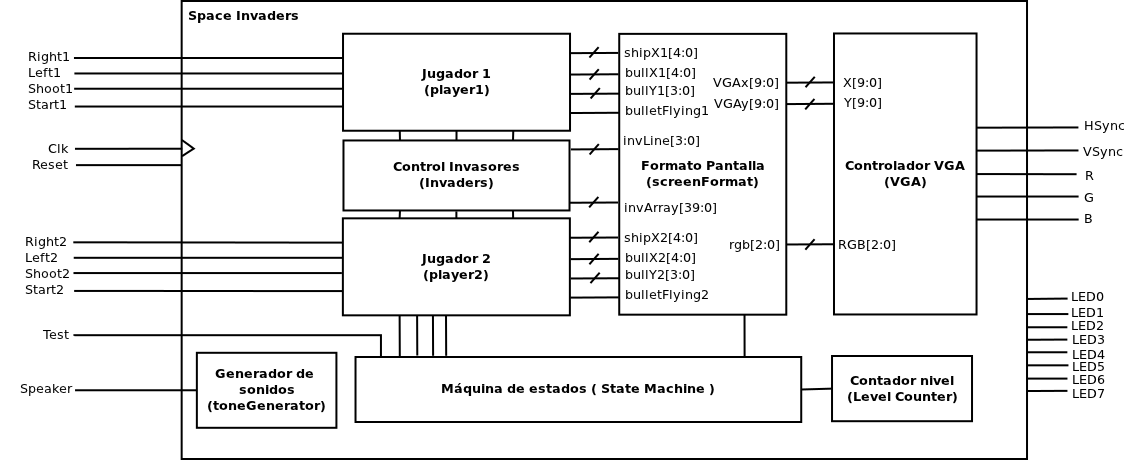
\includegraphics[width=0.8\textwidth]{spaceinvaders.png}
	\caption{Diagrama de bloques del sistema completo. Algunas conexiones no se han indicado por claridad. }\label{fig:spaceinvblock}
\end{figure}

Los bloques básicos incluyen:
\begin{itemize}
	\item {\bfseries Controlador VGA}: Encargado de generar la señal de control de la pantalla.
	\item {\bfseries Formato Pantalla}: Su función es dibujar los distintos elementos del juego en su correspondiente posición de la pantalla.
	\item {\bfseries Control Invasores}: Controla el movimiento de los marcianos y su desaparición tras un disparo.
	\item {\bfseries Control nave}: Controla el movimiento de la nave del jugador.
	\item {\bfseries Control disparo}: Controla el movimiento del disparo.
	\item {\bfseries Detector de flancos}: Convierte la señal de entrada de los pulsadores en un pulso apto para el circuito.
	\item {\bfseries Máquina de estados}: Controla el flujo del juego.
\end{itemize}

Además de esos bloques, se han implementado como mejora los siguientes:
\begin{itemize}
	\item {\bfseries Jugador}: Agrupa varios elementos del jugador, como la nave, el disparo y los detectores de flancos, además de contar la puntuación de ese jugador. Es de gran utilidad para incluir dos jugadores en el juego.
	\item {\bfseries Generador de sonidos}: {\bfseries ??}
	\item {\bfseries Contador de nivel}: sirve para seleccionar la velocidad de juego y dificultad de los marcianos dependiendo de las pantallas ganadas.
	\item {\bfseries Otros}: Además de los bloques anteriores, se han modificado algunos de los bloques básicos para extender su funcionalidad.
\end{itemize}

El mecanismo del juego es el siguiente. Al accionar el interruptor de test en cualquiera de los estados se mostrará en la pantalla un patrón de prueba (tablero de ajedrez) y la partida se reiniciará. El juego se inicia en el estado inicial, en el que se muestra la pantalla de juego estática. En este estado inicial un segundo jugador puede activar la señal de inicio para sumarse a la partida, de forma que pueden jugar 1 ó 2 jugadores. Al pulsar el botón de inicio el jugador 1 el juego se inicia, los invasores comienzan su movimiento y los jugadores pueden moverse y disparar una bala cada vez. 

Si los invasores alcanzan el final de la pantalla, la partida se termina y los jugadores pierden. Si, por el contrario, los jugadores consiguen alcanzar a todos los invasores, superan la pantalla y el nivel se incrementa en 1, pudiendo jugar el siguiente nivel hasta un máximo de 8 niveles, en los que la dificultad de los marcianos y la velocidad de los mismos aumenta. Existen 3 tipos de invasores, verdes, amarillos y blancos, que requieren 1, 2 y 3 disparos respectivamente para morir. Cada disparo acertado aumenta la puntuación de ese jugador en 1 unidad. Si se pierde la partida en cualquiera de los niveles los jugadores deben empezar de nuevo desde el primer nivel (no se dispone de vidas extra).

{\bfseries añadir aquí algo sobre el sonido}
\newpage
